%
%===============>>  ГРУППА 10-1 МОДУЛЬ 5  <<=============
%
\setmodule{5}

%BEGIN_FOLD % ====>>_____ Занятие 1 _____<<====
\begin{class}[number=1]
	\begin{listofex}
		\item
		\begin{minipage}[t]{\bodywidth}
			На рисунке изображён график функции вида \[ f(x)=ax+|bx+c|+d, \] где \(a, b, c, d\) --- целые числа. Найдите корень уравнения \(bx+c=0\).
		\end{minipage}
		\hspace{0.02\linewidth}
		\begin{minipage}[t]{\picwidth}
			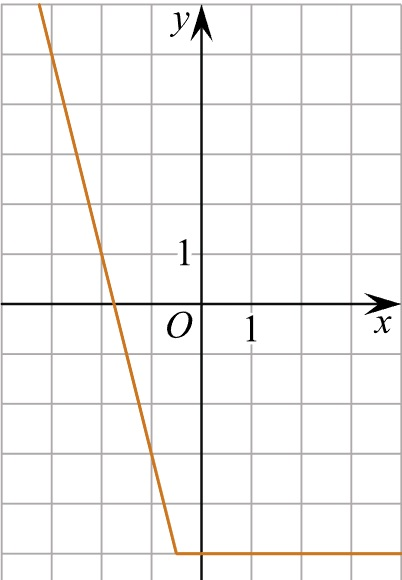
\includegraphics[align=t, width=\linewidth]{\picpath/G101M4H2-6}
		\end{minipage}
		\item
		\begin{minipage}[t]{\bodywidth}
			На рисунке изображён график функции вида \[ f(x)=ax-|bx+c|+d, \] где \(a, b, c, d\) --- целые числа. Найдите корень уравнения \(ax=d\).
		\end{minipage}
		\hspace{0.02\linewidth}
		\begin{minipage}[t]{\picwidth}
			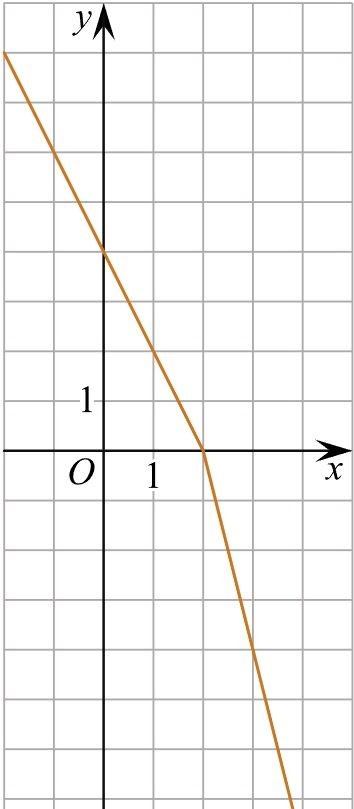
\includegraphics[align=t, width=\linewidth]{\picpath/G101M4H2-7}
		\end{minipage}
		\item
		\begin{minipage}[t]{\bodywidth}
			На рисунке изображён график функции вида \[ f(x)=ax+|bx+c|+d, \] где числа \(a, b, c, d\) --- целые. Найдите корень уравнения \(-ax-3d=10\).
		\end{minipage}
		\hspace{0.02\linewidth}
		\begin{minipage}[t]{\picwidth}
			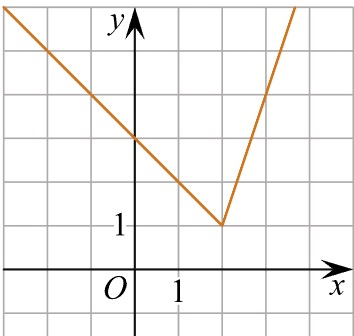
\includegraphics[align=t, width=\linewidth]{\picpath/G101M4C5-7}
		\end{minipage}
%				\item
%		\begin{minipage}[t]{\bodywidth}
%			На рисунке изображён график функции вида \[ f(x)=ax+|bx+c|+d, \] где числа \(a, b, c, d\) --- целые. Найдите корень уравнения \(bx+2c=1\).
%		\end{minipage}
%		\hspace{0.02\linewidth}
%		\begin{minipage}[t]{\picwidth}
%			\includegraphics[align=t, width=\linewidth]{\picpath/G101M4L7-6}
%		\end{minipage}
		\item Два велосипедиста одновременно отправляются в \( 60 \)-километровый пробег. Первый едет со скоростью на \( 10 \) км/ч большей, чем второй, и прибывает к финишу на \( 3 \) часа раньше второго. Найдите скорость велосипедиста, пришедшего к финишу вторым.
	\end{listofex}
\end{class}
%END_FOLD

%BEGIN_FOLD % ====>>_____ Занятие 2 _____<<====
\begin{class}[number=2]
	\begin{listofex}
		%1
		\item
		\begin{minipage}[t]{\bodywidth}
			На рисунке изображён график функции вида \[ f(x)=ax-|bx+c|+d, \] где числа \(a, b, c, d\) --- целые.\\ Найдите корень уравнения \(ax+d=19\).
		\end{minipage}
		\hspace{0.02\linewidth}
		\begin{minipage}[t]{\picwidth}
			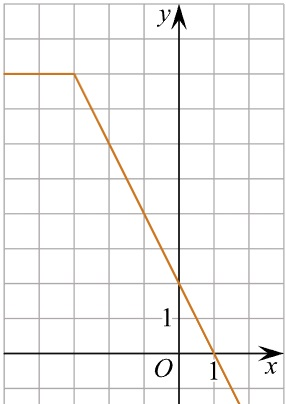
\includegraphics[align=t, width=\linewidth]{\picpath/K-L8}
		\end{minipage}
		%2
		\item
		\begin{minipage}[t]{\bodywidth}
			На рисунке изображён график функции вида \[ f(x)=ax+|bx+c|+d, \] где числа \(a, b, c, d\) --- целые.\\ Найдите корень уравнения \(bx+c=0\).
		\end{minipage}
		\hspace{0.02\linewidth}
		\begin{minipage}[t]{\picwidth}
			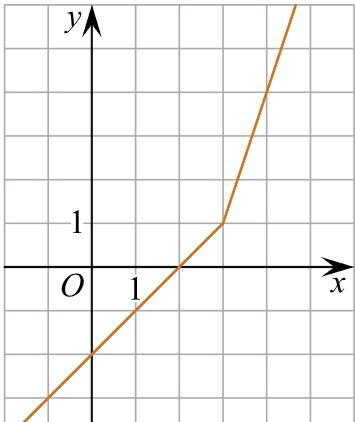
\includegraphics[align=t, width=\linewidth]{\picpath/K-L2}
		\end{minipage}
		%3
		\item
		\begin{minipage}[t]{\bodywidth}
			На рисунке изображён график функции вида \[ f(x)=ax+|bx+c|+d, \] где числа \(a, b, c, d\) --- целые.\\ Найдите корень уравнения \(ax+d=19\).
		\end{minipage}
		\hspace{0.02\linewidth}
		\begin{minipage}[t]{\picwidth}
			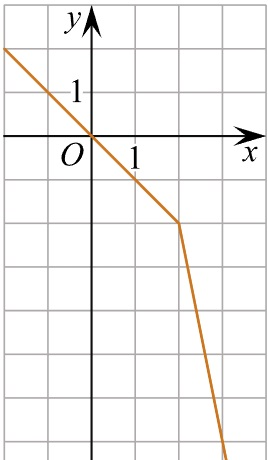
\includegraphics[align=t, width=\linewidth]{\picpath/K-L7}
		\end{minipage}
		%4
		\item
		\begin{minipage}[t]{\bodywidth}
			На рисунке изображён график функции вида \[ f(x)=ax-|bx+c|+d, \] где числа \(a, b, c, d\) --- целые.\\ Найдите корень уравнения \(ax=d\).
		\end{minipage}
		\hspace{0.02\linewidth}
		\begin{minipage}[t]{\picwidth}
			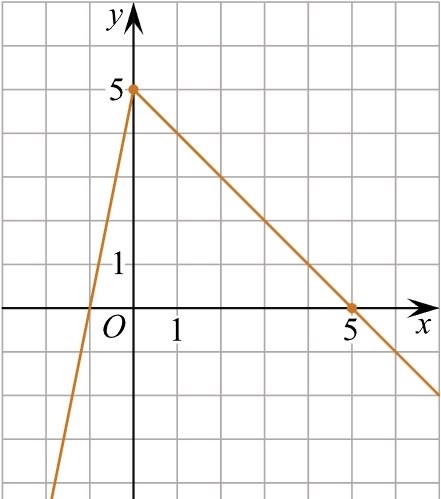
\includegraphics[align=t, width=\linewidth]{\picpath/K-L10}
		\end{minipage}
	\end{listofex}
\end{class}
%END_FOLD

%BEGIN_FOLD % ====>>_ Домашняя работа 1 _<<====
\begin{homework}[number=1]
	\begin{listofex}
		%1
		\item
		\begin{minipage}[t]{\bodywidth}
			На рисунке изображён график функции вида \[ f(x)=ax-|bx+c|+d, \] где числа \(a, b, c, d\) --- целые.\\ Найдите корень уравнения \(ax=d\).
		\end{minipage}
		\hspace{0.02\linewidth}
		\begin{minipage}[t]{\picwidth}
			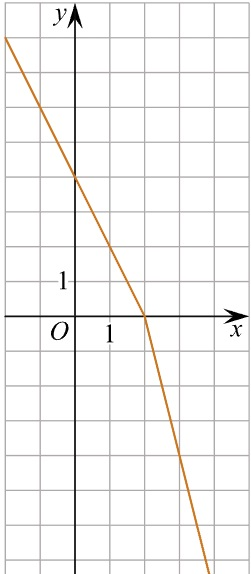
\includegraphics[align=t, width=\linewidth]{\picpath/K-L9}
		\end{minipage}
%		%2
%		\item
%		\begin{minipage}[t]{\bodywidth}
%			На рисунке изображён график функции вида \[ f(x)=ax+|bx+c|+d, \] где числа \(a, b, c, d\) --- целые. Найдите корень уравнения \(ax+2d=12\).
%		\end{minipage}
%		\hspace{0.02\linewidth}
%		\begin{minipage}[t]{\picwidth}
%			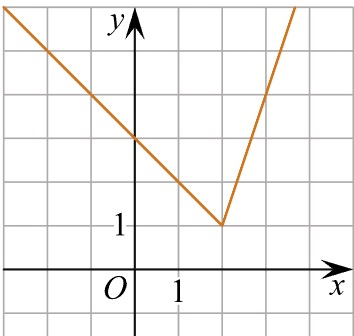
\includegraphics[align=t, width=\linewidth]{\picpath/K-L1}
%		\end{minipage}
		\item Постройте сечение параллелепипеда \( ABCDA_1B_1C_1D_1 \)
		плоскостью, проходящей через следующие точки \( A \), \( C \) и середину \( C_1D_1 \).
		\item Постройте сечение треугольной пирамиды \( DABC \) плоскостью,
		проходящей через середины \( K \), \( L \) и \( M \) ребер \( AD \), \( BD \) и \( BC \).
		\item Решить равнение: \( \sqrt{\dfrac{2x+5}{3}}=5 \)
%		%3
%		\item
%		\begin{minipage}[t]{\bodywidth}
%			На рисунке изображён график функции вида \[ f(x)=ax-|bx+c|+d, \] где числа \(a, b, c, d\) --- целые.\\ Найдите корень уравнения \(ax+d=10\).
%		\end{minipage}
%		\hspace{0.02\linewidth}
%		\begin{minipage}[t]{\picwidth}
%			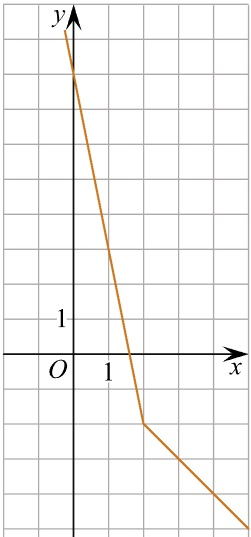
\includegraphics[align=t, width=\linewidth]{\picpath/K-L6}
%		\end{minipage}
%		%4
%		\item
%		\begin{minipage}[t]{\bodywidth}
%			На рисунке изображён график функции вида \[ f(x)=ax+|bx+c|+d, \] где числа \(a, b, c, d\) --- целые.\\ Найдите корень уравнения \(ax+d=5\).
%		\end{minipage}
%		\hspace{0.02\linewidth}
%		\begin{minipage}[t]{\picwidth}
%			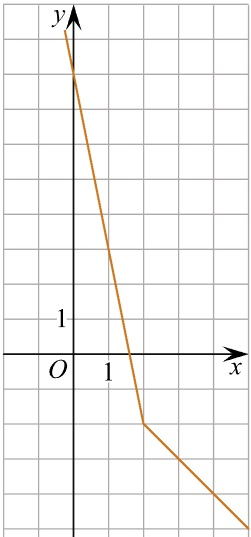
\includegraphics[align=t, width=\linewidth]{\picpath/K-L6}
%		\end{minipage}
%		%5
%		\item Из одной точки круговой трассы, длина которой равна \(14\) км, одновременно в одном направлении стартовали два автомобиля. Скорость первого автомобиля равна \(80\) км/ч, и через \(40\) минут после старта он опережал второй автомобиль на один круг. Найдите скорость второго автомобиля. Ответ дайте в км/ч.
%		%6
%		\item На изготовление \(475\) деталей первый рабочий тратит на \(6\) часов меньше, чем второй рабочий на изготовление \(550\) таких же деталей. Известно, что первый рабочий за час делает на \(3\) детали больше, чем второй. Сколько деталей в час делает первый рабочий?
	\end{listofex}
\end{homework}
%END_FOLD

%BEGIN_FOLD % ====>>_____ Занятие 3 _____<<====
\begin{class}[number=3]
	\begin{definit}
		Сечением фигуры плоскостью является многоугольник, стороны которого принадлежат граням многогранника.
	\end{definit}
	\begin{symrule}
		Соединяйте точки, которые лежат в одной грани (в плоскости этой грани).
	\end{symrule}
	\begin{symrule}
		Плоскость сечения пересекает параллельные грани по параллельным прямым.
	\end{symrule}
	\begin{definit}
		Если некоторая прямая параллельна прямой в плоскости, то она параллельна всей плоскости.
	\end{definit}
	\begin{symrule}
		Если плоскость сечения проходит через прямую,
		параллельную какой-то грани (плоскости), то секущая плоскость
		пересечёт данную грань (плоскость) по параллельной прямой.
	\end{symrule}
	\begin{listofex}
		\item Постройте сечение треугольной пирамиды \( DABC \) плоскостью,
		проходящей через следующие точки:
		\begin{tasks}(1)
			\task \( B \), \( D \) и середину \( M \) ребра \( AC \);
			\task середину \( K \) ребра \( AD \) и точки \( L \) и \( M \), лежащие на продолжениях
			рёбер \( AB \) и \( AC \) за точки \( B \) и \( C \);
			\task середины \( K \), \( L \) и \( M \) рёбер AD, AB и BC;
		\end{tasks}
		\item Постройте сечение параллелепипеда \( ABCDA_1B_1C_1D_1 \)
		плоскостью, проходящей через следующие точки:
		\begin{tasks}(1)
			\task середины рёбер \( AB \), \( AD \) и \( AA_1 \);
			\task \( A \), \( C \) и середину ребра \( A_1B_1 \);
			\task середины рёбер \( AA_1 \), \( AD \) и центр грани \( BB_1C_1C \);
			\task середину ребра \( CC_1 \) и точки \( K \), \( L \), лежащие на рёбрах \( AB \) и \( A_1B_1 \),
			если \( BK : KA= A_1L : LB_1=1 : 2 \);
		\end{tasks}
		\item Точка \(M\) лежит на ребре \(AB\) треугольной пирамиды \(ABCD\), причём \(AM : MB = 1:2\). Постройте сечение пирамиды плоскостью, проходящей через точку \(M\) и середины рёбер \(BC\) и \(AD\).
		\item
		\begin{minipage}[t]{\bodywidth}
			На рисунке изображён график функции вида \[ f(x)=ax-|bx+c|+d, \] где числа \(a, b, c, d\) --- целые. Найдите корень уравнения \(ax+d=-2\).
		\end{minipage}
		\hspace{0.02\linewidth}
		\begin{minipage}[t]{\picwidth}
			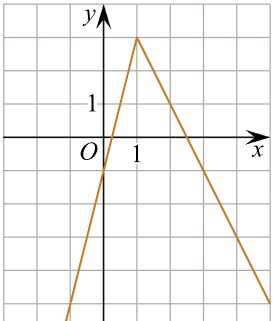
\includegraphics[align=t, width=\linewidth]{\picpath/G101M4C6-8}
		\end{minipage}
%		\item Точка \(M\) — середина ребра \(AD\) треугольной пирамиды \(ABCD\). Точки \(K\) и \(L\) лежат на прямых \(AB\) и \(AC\) соответственно, причём \(B\) --- середина отрезка \(AK\), а \(C\) — середина отрезка \(AL\). Постройте сечение пирамиды плоскостью, проходящей через точки \(M, K, L\).
%		\item Точки \(M\) и \(N\) — середины рёбер соответственно \(AB\) и \(BC\) параллелепипеда \(ABCDA_1B_1C_1D_1\).
%		а) Постройте сечение параллелепипеда плоскостью, проходящей через точки \(M, N, D_1\). б) В каком отношении плоскость сечения делит ребро \(AA_1\)?
	\end{listofex}
\end{class}
%END_FOLD

%BEGIN_FOLD % ====>>_____ Занятие 4 _____<<====
\begin{class}[number=4]
	\begin{listofex}
		\item Основание пирамиды \( SABCD \) --- параллелограмм \( ABCD \).
		Постройте сечение пирамиды плоскостью, проходящей через следующие
		точки:
		\begin{tasks}(1)
			\task \( A \), \( B \) и середина ребра \( SD \);
			\task середины рёбер \( AB \), \( BC \) и \( SC \);
			\task середины рёбер \( AB \), \( BC \) и \( SD \);
			\task центр основания, середину ребра \( SD \) и точку \( M \) ребра \( SA \),
			если \( AM : MS = 1 : 3 \);
		\end{tasks}
		\item Основание шестиугольной призмы \( ABCDEFA_1B_1C_1D_1E_1F_1 \) ---
		правильный шестиугольник \( ABCDEF \).
		Постройте сечение призмы плоскостью,
		проходящей через следующие точки:
		\begin{tasks}(1)
			\task \( A \), \( B \) и \( F_1 \);
			\task \( A \), \( C \) и \( D_1 \);
			\task \( B \), \( E \) и середину ребра \( FF_1 \);
			\task \( B \), \( C \) и \( E_1 \);
			\task \( B \), \( D \) и середину ребра \( FF_1 \).
		\end{tasks}
		\item Диагональ куба равна \( 4 \). Найдите площадь его поверхности.
		\item Дан куб \( ABCDA_1B_1C_1D_1 \). Площадь четырехугольника \( ABC_1D_1 \) равна \( 4\sqrt{2} \). Найдите площадь поверхности куба.
	\end{listofex}
\end{class}
%END_FOLD

%BEGIN_FOLD % ====>>_____ Занятие 5 _____<<====
\begin{class}[number=5]
	\begin{listofex}
		\item Занятие 5
	\end{listofex}
\end{class}
%END_FOLD

%BEGIN_FOLD % ====>>_____ Занятие 6 _____<<====
\begin{class}[number=6]
	\begin{listofex}
		\item Два ребра прямоугольного параллелепипеда, выходящие из одной вершины, равны \(3\) и \(4\). Площадь поверхности этого параллелепипеда равна \(94\). Найдите третье ребро, выходящее из той же вершины и объем параллелепипеда.
		\item Объем прямоугольного параллелепипеда равен \(24\). Одно из его ребер равно \(3\). Найдите площадь грани параллелепипеда, перпендикулярной этому ребру.
		\item Прямоугольный параллелепипед описан около сферы с радиусом, равным \(1\) см. Найдите его объём.
		\item Прямоугольный параллелепипед описан около сферы радиуса \(1\). Найдите его площадь поверхности и объем.
		\item 
		\begin{minipage}[t]{\bodywidth}
			На рисунке изображен многогранник, все двугранные углы многогранника прямые. Найдите его объем.
		\end{minipage}
		\hspace{0.02\linewidth}
		\begin{minipage}[t]{\picwidth}
			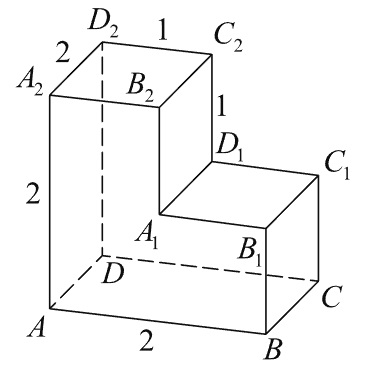
\includegraphics[align=t, width=\linewidth]{\picpath/G101M5L6-1}
		\end{minipage}
		%\item С помощью этого же рисунка найдите расстояние между вершинами:
		%\begin{tasks}(3)
		%	\task \(D\) и \(C_2\),
		%	\task \(B_1\) и \(D_2\),
		%	\task \(D_2\) и \(A_1\),
		%	\item \(A\) и \(C_2\).
		%\end{tasks}
		%\item С помощью этого же рисунка найдите:
		%\begin{tasks}(2)
		%	\task угол \( CAD_2 \),
		%	\task угол \( ABD \),
		%	\task тангенс угла \( B_2A_2C_2 \).
		%\end{tasks}
		\item Даны два прямоугольных параллелепипеда: ребра одного равны \(185 , 185\) и \(37\); а ребра другого равны \(185 , 37,\) и \(37\). Во сколько раз объем первого параллелепипеда больше объема второго параллелепипеда? Сравните площади их поверхностей.
		\item Найдите высоту прямоугольного параллелепипеда, если площади смежных боковых граней равны \(40\) и \(48\) см\(^2\), а объем равен \(240\) см\(^3\).
		\item Постройте сечение прямоугольного параллелепипеда \(ABCDA_1B_1C_1D_1\)
		плоскостью, проходящей через точки \(A, A_1\) и середину \(B_1C_1\).
		\item Найдите площадь боковой и полной поверхностей правильной шестиугольной призмы, сторона основания которой равна \(5\), а высота --- \(10\).
	\end{listofex}
\end{class}
%END_FOLD

%BEGIN_FOLD % ====>>_____ Занятие 7 _____<<====
\begin{class}[number=7]
	\begin{listofex}
		\item Занятие 7
	\end{listofex}
\end{class}
%END_FOLD

%BEGIN_FOLD % ====>>_ Домашняя работа 2 _<<====
\begin{homework}[number=2]
	\begin{listofex}
		\item Дана треугольная пирамида \(ABCD\). Точка \(M\) лежит на ребре \(BC\), причём \(BM:MC = 1:2\). Постройте точку пересечения прямой, проходящей через точку \(M\) и середину ребра \(CD\), с плоскостью \(ABD\).
		\item Основание пирамиды \(SABCDEF\) --- шестиугольник \(ABCDEF\), противоположные стороны \(BC\) и \(EF\) которого параллельны. Точка \(M\) лежит на ребре \(SC\). Постройте точку пересечения прямой \(BM\) с плоскостью \(ESF\).
		\item Основание пирамиды \(SABCD\) --- параллелограмм \(ABCD\). Постройте сечение пирамиды плоскостью, проходящей через следующие точки:
		\begin{itasks}[1]
			\task \(A, B\) и середина ребра \(SD\);
			\task середины рёбер \(AB, BC, SC\);
			\task середины рёбер \(AB, BC, SD\);
			\task середины рёбер \(AB, AD\) параллельно ребру \(SC\);
			\task середины рёбер \(AB, BC, SD\) и точку \(B\);
			\task середины рёбер \(AB, AD, SC\);
			\task центр основания, середину ребра \(SD\) и точку \(M\) ребра \(SA\), если \(AM:MS = 1:3\);
			\task середину ребра \(SA\) и точки \(M\) и \(N\) рёбер \(SB\) и \(SC\), если \(BM : MS = = SN :NC=1:2\)
		\end{itasks}
		\item Точка \(M\) — середина ребра \(AB\) треугольной призмы \(ABCA_1B_1C_1\). а) Постройте сечение призмы плоскостью, проходящей через прямую \(A_1M\) параллельно прямой \(AC\). б) В каком отношении плоскость сечения делит отрезок, соединяющий точку \(B_1\) с серединой ребра \(AC\)?
	\end{listofex}
\end{homework}
%END_FOLD

%BEGIN_FOLD % ====>>_ Домашняя работа 3 _<<====
\begin{homework}[number=3]
	\begin{listofex}
		\item Два ребра прямоугольного параллелепипеда, выходящие из одной вершины, равны \(1, 2\). Площадь поверхности параллелепипеда равна \(16\). Найдите его объём.
		\item Прямоугольный параллелепипед описан около сферы с диаметром, равным \(2\) см. Найдите его объём.
		\item 
		\begin{minipage}[t]{\bodywidth}
			На рисунке изображен многогранник, все двугранные углы многогранника прямые. Найдите его объём.
		\end{minipage}
		\hspace{0.02\linewidth}
		\begin{minipage}[t]{\picwidth}
			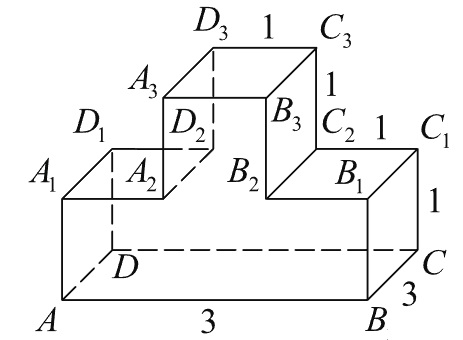
\includegraphics[align=t, width=\linewidth]{\picpath/G101M5L6-2}
		\end{minipage}
		\item Найдите ширину прямоугольного параллелепипеда, если площади смежных боковых граней равны \(22\) и \(60\) см\(^2\), а объем равен \(660\) см\(^3\).
		\item Найдите корень уравнения \(\dfrac{1}{9x-7}=\dfrac{1}{2}\)
		%\item Два ребра прямоугольного параллелепипеда, выходящие из одной вершины, равны \(1, 2\). Площадь поверхности параллелепипеда равна \(16\). Найдите его объем. 
		%\item С помощью этого же рисунка найдите:
		%\begin{tasks}(1)
		%	\task расстояние между вершинами \(B\) и \(D_2\),
		%	\task расстояние между вершинами \(A\) и \(C_3\),
		%	\task найдите тангенс угла \(C_2C_3B_2\).
		%\end{tasks}
	\end{listofex}
\end{homework}
%END_FOLD

%BEGIN_FOLD % ====>>_ Проверочная работа _<<====
\begin{exam}
	\begin{listofex}
		\item Проверочная работа
	\end{listofex}
\end{exam}
%END_FOLD
